So our declared goal is to transform an application, written for a shared memory, single core runtime into a form that is amenable to compilation with Ohua. Also the resulting compiled program should have the following properties:
\begin{enumerate}
    \item The application should have three independent, stateful components, namely a key-value store answering requests, the TCP/IP stack and the device driver. 
    \item Those components can run concurrently, i.e. it is possible to streamline process packages. 
    \item Those components are local to a single executing process each, i.e. no statefully used component is ever send from one process to another.
    \item The final data flow program runs on the M3 operating system and architecture.
\end{enumerate}

To achieve this goal, both smoltcp and Ohua must be adjusted. Therefore, in this chapter we will first describe the structure of our smoltcp application and the necessary changes. Then we will describe how the current functionality of Ohua needs to be adapted and extended. 

\section{Transformations in smoltcp}
\label{sec:ImplSmoltcp}

In its current sequential, single-threaded state, smoltcp makes use of several language features that Ohua's programming model does not support because they cannot be translated into a deterministic concurrent program. The first problem is the sharing of memory references between different components. If these components are executed concurrently, race conditions occur. Roughly speaking, it is therefore necessary to replace all accesses to shared references with explicit data flow.

The second fundamental problem is the current flow of control between stateful components. In a sequential program we can invoke a method on one component \emph{A}, do something on it's state, internally call a method on another component \emph{B} and finish the outer call by maybe changing \emph{A}s state again. \emph{A} and \emph{B} belong to the memory of the same process and the state of \emph{A} as well as the execution state of the outer method are automatically preserved during the call of \emph{B}.
This is what happens when a packet is sent or received using smoltcp in its current form. However, in a concurrent, distributed data flow graph, we cannot realize this bi-directional dependency among stateful components. Why is that? The main problem here is realizing concurrency and state locality at once. We could connect distributed components A and B using blocking connections, i.e. \emph{A} calls \emph{B} and blocks until it receives the result. What we achieve this way is a distributed, sequential program. Another way would be to have \emph{A} send its state along with the call to B and B would return this state along with its answer. So \emph{A} can process the next input and upon receiving an answer it can resume the appropriate state. However, this contradicts the requirement of state locality. In particular when states are large objects e.g. a database state, a training state of a deep neural network or alike, we want them to stay encapsulated in on component.\\
\seflue{Ich finds schwer dem Absatz zu folgen ... vergleichende grafische Darstellungen w\"aren irgenwie als Erg\"anzung hilfreich. Angesichts der knappen Zeit vielleicht eine Idee f\"ur die Verteidigung }
\note{What we do here is also required to support method compilation with Ohua in general}

So to compile to a distributed program with local components of smoltcp, we need to disentangle state dependencies from each other. In the following subsection, we explain how this can be done using a small example key-value store application. We begin with introducing the concrete program and sketching the structure of the target program.

\textbf{The Initial Situation: } In Figure~\ref{fig:oldTopLevel} we see the code for our simple key-value store application. First the required structures, i.e. the \rust{ip_stack}, the \rust{device}, the \rust{store} and some sockets are initialized. Then in the \rust{ip_stack.poll} call the socket and the device are used to send the messages from the sockets to the device and vice versa. Then, depending on the state of the socket, the store answers received messages directly to the socket. Finally the application holds for a time interval determined by a) the current state of the sockets \rust{ip_stack.poll_delay} and b) the current state of the device, represented by waiting for its file pointer \rust{fd} to become available. After that, the interface exchanges messages again.


\begin{figure}[H]
    \centering
    
\begin{minted}[fontsize=\footnotesize]{rust}
fn main() {
    let mut store = Store::default();
    let mut device = TunTapInterface::new("tap0", Medium::Ethernet).unwrap();
    // ... more interface initialization code
    let mut ip_stack = builder.finalize(&mut device);

    let mut sockets = SocketSet::new(vec![]);
    // .. more socket initialization code
    let tcp_socket = tcp::Socket::new(tcp_rx_buffer, tcp_tx_buffer);
    let tcp_handle = sockets.add(tcp_socket);

    loop {
        let timestamp = Instant::now();
        match ip_stack.poll(timestamp, &mut device, & mut sockets) {
            Ok(_) => {}
            Err(e) => {
                debug!("poll error: {}", e);
            }
        }

        let socket = sockets.get_mut::<tcp::Socket>(tcp_handle);
        if !socket.is_open() {
            socket.listen(6969).unwrap();
        }

        if socket.may_recv() {
            let input = socket.recv(process_octets).unwrap();
            if socket.can_send() && !input.is_empty() {
                debug!(
                    "tcp:6969 send data: {:?}",
                    str::from_utf8(input.as_ref()).unwrap_or("(invalid utf8)")
                );
                let outbytes = store.handle_message(&input);
                socket.send_slice(&outbytes[..]).unwrap();
            }
        } else if socket.may_send() {
            debug!("tcp:6969 close");
            socket.close();
        }

        phy_wait(fd, ip_stack.poll_delay(timestamp, &sockets)).expect("wait error");
    }
}
\end{minted}
    \caption{Simplified example of a key-value server application using smoltcp}
    \label{fig:oldTopLevel}
\end{figure}


 Obviously, this code does not meet our compilation requirements. Concrete problems are 
\begin{enumerate}
    \item There are several stateful uses of \rust{socket}, e.g. in \rust{socket.listen(6969)}. However, we do not want those to be visible to the compiler, since they would result in their own, stateful nodes. This is basically a problem of efficient resource utilization, as every node incurs the overhead of an independent process or thread of the target architecture.  
    \item In the call \rust{ip_stack.poll} the \rust{device} is passed as an argument. This means the compiler cannot \emph{see} the device being used as an independent component and will not derive the according code.
    \item The \rust{ip_stack} is statefully called twice inside the loop. This means the compiler will not be able to derive a single node acting on/as the \rust{ip_stack} but instead wil derive a data flow where the \rust{ip_stack} is send from one node using it to the other. 
    \item We cannot simply transfer the mechanism of \rust{phy_wait(fd,...)} to another operating system. For one thing, the function itself is a system call, which means it depends on the operating system. Secondly, \rust{fd} is a file pointer and the handling of pointers and files is also strongly dependent on the target operating system and architecture.
\end{enumerate}

So given this initial code setting and the problems we need to solve to enable the compilation, we can now proceed with describing the actual changes made in this work. 

\subsection{Sketching the Target Structure}

To better understand the transformations described in this chapter, we will figure out the structure of the target program first. We want each of the target components to be used exactly once inside the scope as an object a method is called on. Further we want all implicit state sharing, i.e. the common use of references between components to be eliminated and be replaced by actual explicit message passing. Finally we want function calls, other than the three stateful calls and the initialization of our object to happen outside the compile scope in order to restrict the resulting data flow graph to as few nodes as possible and to generate an efficient program. \\

The first step to get a clearer picture of our goal is to wrap code details the compiler does not need to see into function calls. So as a first step and to get a clearer picture of our target structure, we encapsulate the initialization of components. Also we saw in the original code in Figure~\ref{fig:oldTopLevel} \rust{sockets} being processed, \emph{loaded} with messages by the \rust{store} and than passed to the \rust{ip_stack} along with the \rust{device} for actually processing the TCP/IP packets. So we could figure to use the \rust{sockets} are the vehicle we use for communication among the \rust{ip_stack} and the \rust{store} for now and encapsulate the socket handling in the \rust{store.handle_message} call. Also we let the store application handle the result of \rust{ip_stack.poll}. 
Now our Code looks as follows:

\begin{minted}[fontsize=\footnotesize]{rust}
fn main() {
    let (mut store_app, mut sockets):(App, SocketSet) = init_app_and_sockets();
    let (mut ip_stack, mut device, fd):(Interface<'static>, TunTapInterface, RawFd) = 
      init_stack_and_device();

    loop {
        let timestamp = Instant::now();
        
        let (poll_result, sockets_polled) = 
          ip_stack.poll(timestamp, &mut device, sockets);

        let sockets_loaded = store_app.handle_sockets(poll_result, sockets_polled);

        sockets = 
          phy_wait(
            fd, 
            ip_stack.poll_delay(timestamp, sockets_loaded))
            .expect("wait error");
    }
}
\end{minted}

Now to get an idea of the target structure without going to much into detail, we make the following assumptions: \\
i) We assume for the time being that there is a simple control flow inside \rust{ip_stack.poll} going from the \rust{ip_stack} to the \rust{device} for sending, back to the \rust{ip_stack}, and\\
ii) We know that the \rust{phy_wait} call takes an input from the device, namely the file pointer \rust{fp} and an input from the \rust{ip_stack}, namely a waiting time from the sockets and halts the loop for a certain interval before the \rust{ip_stack} can poll again. Given this structure, we assume we can prepend the calls involved in \rust{phy_wait} to the execution of \rust{poll} itself. 
Applying this assumptions, we get a control flow as depicted in Figure~\ref{fig:mainLoopOriginal}. We see an inner loop among the \rust{ip_stack} and the \rust{device} and an outer loop among the \rust{ip_stack} and the \rust{store}. As smoltcp can be used heapless, all process steps act on shared references instead of moved owned values.

\begin{figure}[H]
    \centering
    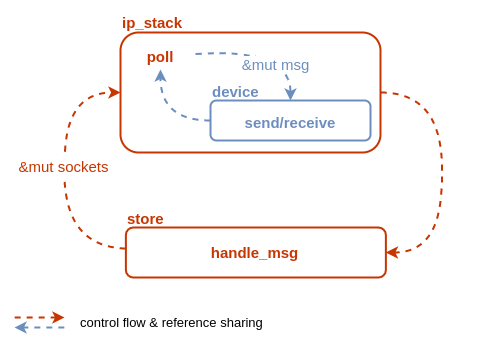
\includegraphics[height=5cm]{figures/outer_scope_before.png}
    \caption{Simplified structure of the original process loop}
    \label{fig:mainLoopOriginal}
\end{figure}

Now for this simplified structure, we can already see what needs to be done to achieve our target characteristics. We need to move the inner loop inside \rust{poll} into the main scope.
For now we assume we had simply split \rust{poll} into parts e.g. asking the \rust{device} for availability, waiting before poll, preparing packets and sending them. And we create a method \rust{ip_stack.process()} that can execute either of those parts, based on the input.
Also we change all method signatures to explicitly return and except values instead of references.This directly results in the structure shown in Figure\ref{fig:mainLoopTarget}. 

\begin{figure}[H]
    \centering
    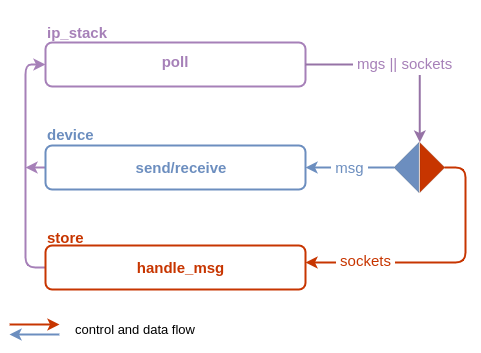
\includegraphics[height=5cm]{figures/outer_scope_target.png}
    \caption{Simplified structure of the target process loop}
    \label{fig:mainLoopTarget}
\end{figure}

Without looking at the inner workings of poll in detail, we can already recognize essential properties of the target program here

\begin{enumerate}
    \item The final structure is a nested loop.
    \item Since we want to use only one method call for the \rust{ip_stack}, it must return a type which can be either an input for the \rust{device} or the \rust{store}.
    \item The calls to \rust{device} or the \rust{store} must return a common type that \rust{ip_stack.poll} accepts\footnote{you could also return different types. However, then an additional node would be needed to convert them to a common type}.
    \item In the original structure, the \rust{device} was called inside the \rust{poll} function. Therefore, after each call to \rust{device}, the control flow automatically returned to the execution state of \rust{poll}. Now the substeps of \rust{process} are individual method calls. That means we will need a way to transfer the execution state of \rust{poll} from one call to the next. 
\end{enumerate}

In the next sections, we will first take a closer look at the control flow in poll. We will describe how to implement inner loop extraction and what problems arise when converting reference arguments to moved objects, i.e. call by reference to call by value.

\subsection{Encapsulating the Socket Handling}
\label{subsec:SocketHandling}
In sketching the target program, the first change made to the original code was to encapsulate as much of the logic as possible into either the states or the initialization functions. As a first guess, the socket handling i.e. checking if sockets are open, setting them to listening state etc. was encapsulated in the \store{.handle_sockets} call. The problem with this decision is that the actual \rust{SocketSet} type contains lifetime bound references, meaning they do not implement \rust{Clone} and we cannot just replace passing them by reference with actually moving them. Implementing a custom, owned version of the \rust{SocketSet} would be a remedy for this problem. However, the internal references are actually different buffer types used in the sockets and manipulated in many places in the core logic of smoltcp. This means that implementing a custom, owned \rust{SocketSet} type would not only result in extensive changes, but would also negatively affect the efficiency of the program. The other option is to not send the sockets, but only the required information among components. What this required information is, depends on how each of the components involved interacts with the sockets. For our example key-value store application, the interaction between sockets and \store{} is fairly simple. The \store{} receives a message from a socket and answers it. As we will later see, the interaction between the \stack{} and the sockets is rather involved. So instead of having a free-floating \rust{SocketSet} in the main scope, we make it part of the \stack{} upon initialization. This also means, we need to move the code for handling the sockets into the \stack{} as well and return to the \store{} not directly after polling, but when a socket is processed. We will discuss how this is done in Section~\ref{}\todo[inline]{Where?!}. The main point here is to illustrate the problem of designing the interfaces between components, if they are not clearly defined in the first place. A less simple case could have involved, for instance, conditional opening or closing of sockets by the \store{} based on concrete messages, time, traffic volume etc. and would have required an extended message interface between the \stack{} and \store{} and potentially a replication of the sockets in both components updating each other via this interface. In general, this information cannot be meaningfully derived from static, purely syntactic information from high-level language input code.

\subsection{Refactoring Packet Sending}
The next step is to refactor the \rust{poll} method. We need to bring the stateful usage of the \dev{} into the compile scope and create a single \emph{entry method} the three 
components use to call each other. This \emph{entry method} will internally dispatch each call to the actual method, or generally code to be called on the states.\\

The code of \rust{poll} is depicted in Figure~\ref{fig:pollCode}. The method itself contains a loop calling \rust{socket_egress} which executes sending packets to the \rust{device} and \rust{socket_ingress} which receives packets and distributes them to the \rust{sockets}. As long as there are packets send or received in each loop, \rust{poll} continues. \\

\begin{figure}[H]
    \centering
    
\begin{minted}[fontsize=\footnotesize]{rust}
pub fn poll<D>(
    &mut self, timestamp: Instant,
    device: &mut D, sockets: &mut SocketSet<'_>,
    ) -> Result<bool>
    where
        D: for<'d> Device<'d>,
    {
        self.inner.now = timestamp;
        let mut readiness_may_have_changed = false;

        loop {
            let processed_any = self.socket_ingress(device, sockets);
            let emitted_any = self.socket_egress(device, sockets);
            if processed_any || emitted_any {
                readiness_may_have_changed = true;
            } else {
                break;
            }
        }
        Ok(readiness_may_have_changed)
    }
}
\end{minted}
    \caption{Simplified code of the \rust{ip_stack.poll} method}
    \label{fig:pollCode}
\end{figure}

As we can see the \dev{} reference is passed further down into two method calls, the receiving method \rust{socket_ingress} and the sending method \rust{socket_egress}. We will start with explaining the transformations in \rust{socket_egress}, because it is structurally  more complex than \rust{socket_ingress} and therefore better suited to demonstrate all necessary transformation steps.

\subsubsection{Bringing \dev{} calls into scope}
\label{subsec:DeviceLifting}
Figure~\ref{fig:egressCode} shows how sending packets proceeds as a loop over the socket items. If a \rust{socket} can send, its \rust{socket.dispatch} method is called passing a reference to the \stack{} and the \rust{respond} closure. As our example works with TCP sockets, inside \rust{dispatch} the \rust{socket} prepares a TCP packet and passes it to the \rust{respond} closure. This closure will then try to get a sending token from the \dev{} and pass the token and the TCP packet. The token is basically a direct reference to the sending buffer of the \dev{}. Finally inside the \rust{inner.dispatch} call of the \rust{stack} will wrap the TCP packet into a network representation e.g. an Ethernet frame and directly write that packet into the device buffer using the token.\\
 
\begin{figure}[H]
    \centering
    
\begin{minted}[fontsize=\footnotesize]{rust}
fn socket_egress<D>(&mut self, device: &mut D, sockets: &mut SocketSet<'_>) 
-> bool
    /*where*/
{
    let Self {
        inner,
        ..
    } = self;
    let mut emitted_any = false;
    for item in sockets.items_mut() {
        if ! can_send(item, inner.now) {
            continue;
        }

        let mut neighbor_addr = None;
        let mut respond = |inner: &mut InterfaceInner, response: IpPacket| {
            neighbor_addr = Some(response.ip_repr().dst_addr());
            let token = device.transmit().ok_or_else(|| {
                /*logging*/
                Error::Exhausted
            })?;

            inner.dispatch_ip(token, response, None)?;
            
            emitted_any = true;

            Ok(())
            };

        let result = match &mut item.socket {
            Socket::Tcp(socket) => socket.dispatch(inner, |inner, response| {
                respond(inner, IpPacket::Tcp(response))
            }),
            // .. other socket types
        };
        
        match result {
            // stop looping if the device was exhausted
            // update socket if adress was wrong
        }
    }
    emitted_any
}
\end{minted}
    \caption{Simplified code of the \stack{.socket_egress} method}
    \label{fig:egressCode}
\end{figure}

 The \dev{} is used twice in this method. Once for receiving a token in the \dev{.transmit()} call, a second time implicitly when this token is used to pass a packet to the device. This happens inside \stack{.inner.dispatch_ip}. Both of this calls happen inside the \rust{socket.dispatch} method. If we look into this method and inline the code of the \rust{response} closure we get the following structure: 
 
\begin{minted}[fontsize=\footnotesize]{rust}
//socket.dispatch(...)
    /*check socket state*/
    if /*a packet can be produced*/{
        let packet = /*produce packet*/;
        neighbor_addr = Some(response.ip_repr().dst_addr());
        let token = device.transmit().ok_or_else(|| {
            /*logging*/
            Error::Exhausted
        })?;
        inner.dispatch_ip(token, response, None)?;
        emitted_any = true;
        Ok(())
        /* 
        if no error occured, update socket state
        using the packet information        
        */
    } else {
         return Ok(())
    }                    
\end{minted}

The method starts with a preparation phase were the socket state is checked. If no packet can be produced, it returns with \rust{Ok(())}. If a packet is produced, a token is required and if successful the packet is sent. \seflue{Satz noch b\"uschen unklar. Im Code steht irgendwas von device.transmit ... will man da noch etwas mehr drauf eingehen? Ansonsten zumindest "and if successfully created the packet is sent"} Afterwards the socket state is updated using information from the packet. If any of the steps fail, the control flow returns an error to the outer scope i.e. to the sending loop. 

\todo[inline]{Find better Name}
\textbf{Refactoring Packet Processing}

To lift device usage into compile scope, we need to inline the content of \rust{socket.dispatch}. This means we refactor a function scope i.e. a separate stack frame to a simple scope in the outer stack frame. Scopes are expressions in Rust. So there are two different ways of returning values from scopes. One is to simply end the scope with an expression. In this case, the scope simply returns the value of that last expression to the outer scope. The second is to use explicit \rust{return} or \rust{?}. They will not only return a value or an error to the surrounding scope, but leave the current stack frame. \\

 So to inline function with early returns or \rust{?}, we need to refactor the early returns to conditional execution i.e. we need to 
 \begin{enumerate}
     \item instantiate a \rust{let result;} at the beginning of the method and whenever either a \rust{return x} or a \emph{expression}\rust{?} appears
     \item replace any returning statement including the final return by binding the potential early return values to the \rust{result} variable, in our example for instance \rust{result = inner.dispatch_ip(token, response, None);}
     \item wrap every subsequent code into a conditional and, 
     \item return the assigned \rust{result}
 \end{enumerate}
\todo[inline]{reference further details in the 'general learnings' or 'not yet supported syntax' section if I have time to spell it out}. 
Now we can safely inline the code. \\
\todo[inline]{figure for inlined code}
\todo[inline]{learnings \means refactoring early returns needed for inlining, otherwise inlined code must comply prog. mod.}

After lifting \rust{socket.dispatch} into scope, the steps before and after the device usage can be re-encapsulated into package pre-processing \rust{socket.dispatch_before} and the socket post-processing and after sending \rust{socket.dispatch_after}. Thereby we see another refactoring problem. When we split execution steps into different functions. In the original code, the 'packet' i.e. the two representations where used in emit and afterwards to update the socket without any referencing or cloning. This was possible, because they implement \rust{Copy} and can therefor be implicitly duplicated. This still works when we inline the socket.dispatch code because still any processing of the packet happens in a single, now extended stack frame. However, it stops working as we re-encapsulated packet handling before and after sending. The reason is that with that re-encapsulation the frame producing the packet (i.e. the pre-process call) is gone, when we want to send it. \\
\note{This would also happen if we did not re-encapsulate but left the code inside poll. The reason is that in any case the steps will be interrupted by a call to the device i.e. by leaving the current stack frame}

To fix this problem, we introduced a heap-allocated version of the package data type. Also, pre-processing now returns two copies of the packet so that one can be used for sending and one for post-processing the socket. 
\note{This is a general problem when we want to make sequential code concurrent or even distributed. In the first case, types need to be transferable from one function stack. Ohua cannot recognize, nor can we automatically implement something like copy, clone or serialization for 
types. Before we assumed that arguments are always passed by value and 
that serialization in the chosen backend is available for all types used as arguments in the compile scope i.e. all types that are send among nodes later. If we tried to implement refactorings/transformations in the compiler that a) split functions or b) bring code into scope that wasn't before, we need to extend this assumption to all code possibly affected by the transformation}
\todo[inline]{figure for refactored code}
\todo[inline]{Note that this refactoring need to happen on the implementers of the socket trait individually, because we need to split concrete implementations of dispatch}


\textbf{Refactor token usage}
Now we need to eliminate the implicit use of the \dev{} inside \stack{.inner.dispatch_ip(token, response, None)}. The sending \rust{token}, passed to this method contains a reference to the \dev{}s sending buffer. So the function as it is violates two requirements by using shared references among components and using one component implicitly inside the other.
Contrary to packet processing, this method ends with the call to the device, meaning there are no state changes occurring after the sending and except the sending result, nothing depends on the actual device behavior. This means, we can separate the packet preparation inside \stack{.inner.dispatch_ip(token, response, None)}, from the effective packet sending in the device, making both steps local to their component. For the \stack{} we provided a local implementation of the sending token. Like the original token, the \rust{LocalToken} holds a reference to a buffer and implements the expected \rust{token.consume} method. Also we replaced the direct call to \stack{.inner.dispatch_ip}, by a wrapper function \stack{.inner.dispatch_local}. That function instantiates a local sending token, executes \stack{.inner.dispatch_ip} and returns the token buffer
containing the packet. On the other hand the device needs an explicit sending method, instead of an implicit call via the token. This new \dev{.send} method basically needs to call the \rust{token.consume} method on a given token, with a given packet. Therefor we do not need to have specific implementations for implementers of the \rust{Device} trait, but can implement \rust{send} directly on the trait. The method \rust{token.consume} does not take a packet, but a closure processing a packet and copying it into a given buffer. Both already happened in the \stack, so we only need a closure that copies the given packet into the actual device buffer. Finally, with respect to our target architecture there is no particular use in requesting and returning actual tokens to the device any more. In a distributed system, file pointers as contained in the tokens cannot trivially be send among components. Therefor, instead of sending tokens we only request them locally in the device when needed and send \rust{Result<()>} to the \stack{} instead. Hence the implementation of the sending function looks as follows:

\begin{minted}[fontsize=\footnotesize]{rust}
pub trait Device<'a> {
    type RxToken: RxToken + 'a;
    type TxToken: TxToken + 'a;
    // ... 
    
    fn send(&'a mut self, timestamp:Instant, packet:Vec<u8>) -> Result<()> {
        let sending_result
            // Request a token locally
            = self.transmit().ok_or_else(|| {
                        net_debug!("failed to transmit IP: {}", Error::Exhausted);
                        Error::Exhausted
                    }).and_then(|token|
                    // copy the packet to the devices sennding buffer
                   token.consume(timestamp, packet.len(),
                     |buffer| Ok(buffer.copy_from_slice(packet.as_slice()))));
        sending_result
    }                 
\end{minted}

\note{The functional split between device and \stack{} can hardly be derived  automatically and in particular statically. Actually I don't think its possible. What needs to be understood by the compiler is 1. there are no state changed in the interface depending on the device reaction 2. tokens contain references to the device i.e. to buffers, file pointers etc. 3. we can split the closures passed to token\_consume into 'preparing a packet and copying it to a local buffer' and 'copying it to the actual buffer'. We also cannot just send the closures. What might be possible is to 1. analyze what arguments from the ipstack the closure takes, 2. send those arguments to the device and 3. have the actual closures stored as functions in the device and execute them. Not quite clear if this would work ... Device would need to know which closure to execute, what happens if they are nested etc. pp.}

\subsubsection{Refactor to Message Passing}

We inlined the code for \rust{socket_egress} into \rust{poll} and lifted the usages of the \dev{} into the scope of the \rust{poll} function. This also means that the control and data flow for sending are now explicit in the \rust{poll} function. Figure~\ref{fig:egressInlinedFlow} shows the principle structure of the sending loop at this stage. The actual code at this point can be found in the Appendix~\ref{appFig:egressInlinedOriginal}. As indicated by dashed and solid errors in the graph, the control flow and the data dependencies of the individual steps are not congruent. In particular the currently processed \rust{socket} is needed in multiple steps in the \stack{}, but not needed by the \dev{}. 

\begin{figure}[H]
    \centering
    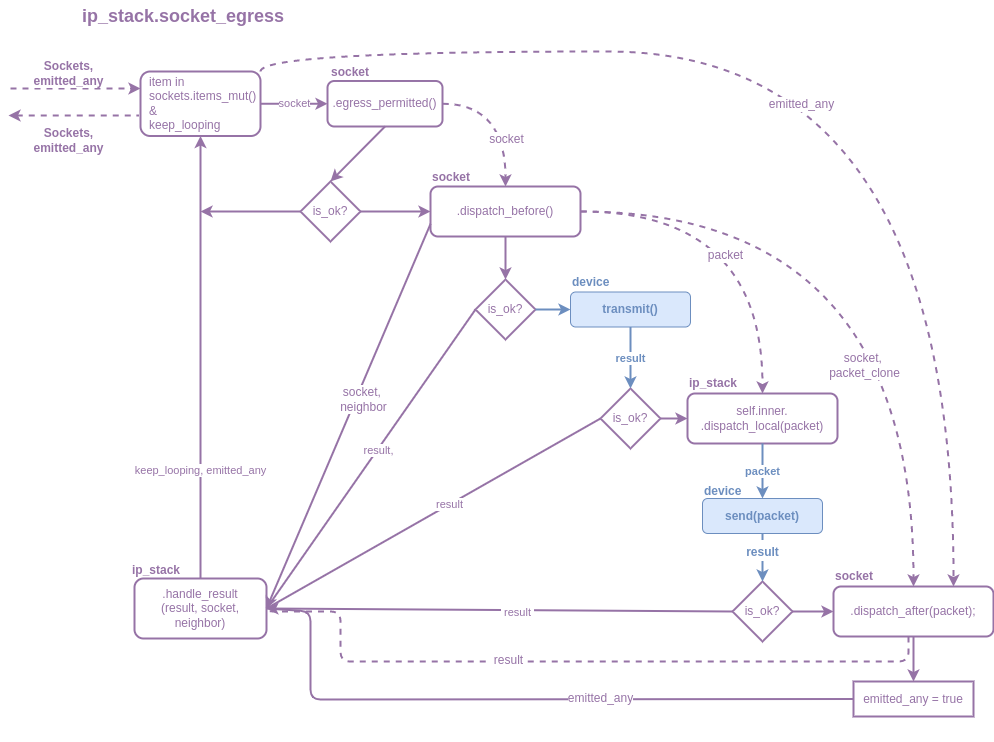
\includegraphics[scale= 0.36]{figures/egress_inlined_detail.png}
    \caption{Structure of the packet sending loop after lifting all device usages into scope. 
    Solid arrows indicate actual control flow, dotted arrows indicate data dependencies}
    \label{fig:egressInlinedFlow}
\end{figure}

\textbf{Refactoring control flow}

Currently the sending loop happens entirely inside or above the stack frame of \rust{poll}. That's why it is possible to use data references and resume execution automatically after the \dev{} is called. We need to refactor the loop such that we can return the frame of the main function when the \dev{} is called and resume the execution inside the \stack{} afterwards. As method calls of the two components are interleaved, we cannot just merge the calls of each component i.e. call the \stack{} to get a packet, call the \dev{} to send it and modify the \stack{}s state again based on the \dev{}s response\footnote{Actually this is an opportunity if state changes in each component are either idempotent or ordered i.e. implemented as Conflict-Free Replicated Data Types. Both is not the case here.}. This necessarily means, we need to split the execution of \rust{poll} into several method calls and we need to preserve the state of execution and the state of variables inside \rust{poll} from one sub-call to the next. 

When we split the \stack{.poll} method, or in general any method into separate \emph{sub-methods}, we have two options to transfer data from one call to another. One is pass them explicitly, the other one is to make them part of the state. Serialization is generally expensive and also in terms of security and process isolation, it is desirable to only send data around that is actually needed in other components. Analyzing the data dependencies between the \stack{} and the \dev{}, it is obvious that the only arguments the \dev{} calls require are the packet to send and, in the actual implementation, a timestamp and the length of the packet. So except for the packet no data needs to leave the \stack{} towards the \dev{}. We will therefore only integrate the packet into the explicit data flow, and preserve the state of other variables in the state of the \stack{}.\\

A common obstacle in both data handling options is the elimination of reference usage. As explained in Section~\ref{subsec:Rust} Rusts type system will point to a problem, when we try to share references among different stack frames. By splitting the original \stack{.poll} method, we execute code that was supposed to run in one stack frame in multiple frames. This means we cannot simply use the data types of the original program. In particular, regardless if we send data or store them in a state between function call, they must not use references among each other. This is obvious for serialized data, as references serialized and send to processes potentially running on a different machine loose their relation to memory. For the case of data stored in a state, consider the following example from our problem. The sending loop is an iteration over the \rust{sockets}. So at the point, where a packet is produced, there are four references to the same memory location in scope namely i) the sockets ii) the iterator on the sockets iii) the current socket and iv) the packet, which actually is a reference to memory inside the socket until it is finally send. As mentioned before, packets need to be become an owned data type to be sendable to the \dev{}. Which eliminates the fourth reference. However, we also need to store the state of iteration and the current socket in the state, without references to the sockets. It is in general not possible to return a \rust{struct} with fields referencing each other in Rust, because the consistency of references cannot be guaranteed\footnote{Actually there are ways to achieve memory consistency across function calls in Rust using e.g. the \rust{std::pin} module. However, they are not applicable to other languages so we do not consider them here.}. In particular we cannot have a socket, referencing an iterator, referencing the sockets in our current state, since any of those reference could become independently invalid leaving dangling references. \\

The problem was solved by implementing an owned representation of the iteration state. As shown in, we integrated the current state of \stack{.socket_egress} as a separate, optional field to the \stack{}. Instead of saving an iterator and a reference to the current socket, only an index of the current socket in the socket set is stored. The socket itself must be retrieved in ever step using it. This also implied that we need to rewrite the iteration on the socket set. Instead of using the given \rust{Iterator} implementation, we implemented iteration over the size of the socket set, starting at the currently saved index. We did the same for the other intermediate results of the original method \rust{neighbor} and \rust{packet} and \rust{address}. The resulting definition of the \stack{} data type is shown below. 

\note{What we can learn here are two things a) a lambda lifting for method may include turning enclosed values to part of the state instead of explicit arguments and b) as long as the compiler is not smart enough to transform references to owned data (which has quite some implications on the code structure) we need to extend the requirement of 'no shared refs, no calls on refs, no refs anywhere in scope anyway' to all the code the compiler might touch.}

\begin{minted}[fontsize=\footnotesize]{rust}
struct Interface<'a> {
    ..,
    egress_state: Option<EgressState<'a>,
}
struct EgressState<'es>{
    sockets_during_egress: Option<SocketSet<'es>>,
    current_index: Option<usize>,
    current_neighbor:Option<Address>,
    current_presend_packet: Option<IpPacketOwned>,
    current_postsend_packet:Option<IpPacketOwned>
}
\end{minted}

Now the control flow needs to be refactored, such that the device is called in the main scope and \dev{} and \stack{} have each only one method call visible to the compiler. This method will be \emph{entry point} of both states and internally dispatch the call to the required code. We will call the method \rust{process_call} and start by defining it on the \dev{}. \\

Intuitively \rust{process_call} would be a higher-order function. Specifically, instead of calling the \dev{} directly, \rust{poll} would return the functions \rust{transmit} or \rust{send} including the necessary arguments. The device would then be called with \dev{.process_call(fn, [args])}. However, higher-order functions are not a viable solution here. This is for two reasons. Firstly we envision to send the functions to be called by \rust{process_call} from one component to the other. But function references are, with some exceptions, not serializable and sendable in distributed scenarios. Secondly we also need to pass the arguments for those called functions to \rust{process_call} so we would need to derive a common sum type to represent all possible function arguments.

The solution to this is called defunctionalization. It is a known transformation used in compilers to transform higher-order functions \cite{reynolds1972definitional}. Instead of sending function references, a sum data type representing all possibly called functions is defined. In Rust we can use \rust{enum}s for this purpose. This \rust{enum} data type also allows us to integrate the arguments called per function so the \rust{enum DeviceCall} looks as follows for the sending loop: 
\begin{minted}[fontsize=\footnotesize]{rust}
#[derive(Debug, Eq, PartialEq, Clone)]
pub enum DeviceCall{
    Transmit,
    Consume(Instant, Vec<u8>),
}
\end{minted}

We merge control flow and data flow here so the return type will be the union of the return types of all functions that might be called, wrapped in the respective next step of execution. In case of the \dev{}, the next step of execution will be a the next part of the \rust{poll} function to be executed. Therefor we define \dev{.process_call} as follows:
\begin{minted}[fontsize=\footnotesize]{rust}
pub trait Device<'a> {
    // ...
    
    fn process_call( &'a mut self, call: DeviceCall
    ) -> InterfaceCall
    {
        match call {
            DeviceCall::Transmit
                => InterfaceCall::InnerDispatchLocal(self.transmit()),
            DeviceCall::Consume(timestamp, packet)
                => InterfaceCall::MatchSocketDispatchAfter(self.send(timestamp, packet)),
    }
}
\end{minted}

In principle, each \dev{.process_call} now returns a continuation in the \stack{}.\\

For the \stack{}, the implementation of \rust{process_call} and the \rust{enum InterfaceCall} is slightly more involved. Contrary to its implementation on the \dev{}, the \stack{.process_call} method will need to call sub-sections of the the \stack{.poll} method. We will consider the simplified pseudocode version shown below for now, to illustrate the principles applied. In the code below, borders of basic blocks, i.e. points the control flow could jump to are marked and given names, because they are needed for the transformation. 

\begin{minted}[fontsize=\footnotesize]{rust}
impl Interface {
    // 1st jump => InitSimplePoll
    fn simple_poll(&mut self, sockets: &mut SocketSet, device: &mut Device) -> bool {
        let mut something_changed = false;
        let mut result: SmoltcpResult<()>;
        // Jump here 2nd => StartSendLoop
        for socket in sockets {
            // Jump here 3rd => GetNextPacket
            let next_packet = self.maybe_get_packet(socket);
            if next_packet.is_ok() {
                result = device.send(next_packet);
                something_changed = result.is_ok();
            } else {
                result = next_packet.as_err()
            }
            // Jump here 3rd => HandleResult
            self.handle_result(result)
        }
        something_changed
    }
}
\end{minted}

Now the transformation from \stack{.simple_poll} to \stack{.process_call} would proceed as follows. First the basic blocks are identified. From those blocks, a corresponding \rust{enum InterfaceCall} is defined representing each of them. If a block uses results from the \dev{}, this results are part of the constructor of its \rust{InterfaceCall} representation. For our simple example this would yield the following \rust{enum}:

\begin{minted}[fontsize=\footnotesize]{rust}
enum InterFaceCall<'a> {
    InitSimplePoll(SocketSet<'a>),
    StartSendLoop,
    GetNextPacket,
    HandleResult,
}
\end{minted}

The \stack{.process_call} is again essentially a \rust{match} expression on the given call. The arms of the matches wrap the respective parts of \rust{simple_poll}. The next modification we need, is to augment every such arm with statements to restore the original environment of each block inside the match arm. We stored the variable state inside the state of the \stack{} as described before, in this trivial example we assume to set them directly as filed of the \stack{}. However, the code in the branches might still use references to the variables and we need to respect rusts borrowing rules, so we cannot generally replace any direct variable use \rust{f(x)} by \rust{f(self.x)}. So we add statements to get and set the stored variables in each block before the code and before each \rust{return} statement respectively. Finally we replace calls to the device by statements returning the respective \rust{DeviceCall} and jumps to other blocks by the corresponding call of \stack{.process_call(next_block_call)}. The actual return statement of \rust{simple_poll} remains unchanged. So the return type of this simplified \stack{.process_call} is \rust{Either<DeviceCall, bool>} and looks as follows. 

\begin{minted}[fontsize=\footnotesize]{rust}
    fn process_call(&mut self, call: InterFaceCall) -> Either<DeviceCall, bool> {
        match call {
            InterFaceCall::InitSimplePoll(sockets) => {
                // set variables something_changes, result, sockets and index
                return self.process_call(StartSendLoop)
            },
            InterFaceCall::StartSendLoop => {
                // get socket and socket_index
                if socket_index+1 < sockets.size() {
                    let socket_index = socket_index+1;
                    // set sockets and socket_index
                    return self.process_call(GetNextPacket);
                } else {
                    // set sockets and socket_index
                    return Either::Right(self.something_changed);
                }
            },
            InterFaceCall::GetNextPacket => {
                let next_packet = self.maybe_get_packet();
                    if next_packet.is_ok() {
                        return Either::Left(DeviceCall::Send(next_packet))
                    } else {
                        self.result = next_packet.as_err();
                        return self.process_call(HandleResult)
                    }
            }
            InterFaceCall::HandleResult => {
                self.handle_result();
                return self.process_call(StartSendLoop)
            }
        }
    }
\end{minted}

The actual implementation of \stack{.process_call} is obviously more complex, but was build in the same transformation steps. 

\todo[inline]{Find better title or reorder}
\subsection{Refactoring Packet Receiving -- Completing the \rust{poll} loop}
Just like sending, receiving is triggered in the \stack{.poll} method. The main aspects of \stack{.socket_ingress()} are depicted in Figure~\ref{fig:socketIngressCode}. In a while loop, the \stack{} tries to receive packets from the \dev{}. In this case packets are represented by a token pair. The receive token \rust{rx_token} contains a buffer holding the received packet, the send token \rust{tx_token} may be used to directly return an answer to the \dev{}. During initialization, the transport medium used by the \dev{} is saved in the \stack{}. By matching on the current transport medium the method to unwrap the outer most layer of the packet is determined, in this case \rust{process_ethernet(sockets, &frame)}. Using the reference to the sockets the function determines which socket the packet should be dispatched to. Next packet is processed by the socket and copied into its receive buffer. From there it can later be retrieved and passed to the \store{}. The socket may also produced a direct answer, for example as part of the TCP protocol. If so this answer is dispatched as discussed before for the sending loop using the \rust{tx_token} as a reference to the device. So in essence the \dev{} is used three times here. First time explicitly for receiving, the second and third time implicitly by accessing its receiving and sending buffer via the tokens.
\begin{figure}[H]
    \centering
\begin{minted}[fontsize=\small]{rust}
fn socket_ingress(&mut self, sockets:&mut SocketSet) -> bool {
    // ... 
    while let Some((rx_token, tx_token)) = device.receive() {
        if let Err(err) = rx_token.consume(inner.now, |frame| match
            inner.caps.medium {
                Medium::Ethernet => match inner.process_ethernet(sockets, &frame) {
                    Ok(response) => {
                        processed_any = true;
                        if let Some(packet) = response {
                            if let Err(err) = inner.dispatch(tx_token, packet) {/*log Send Error*/}
                        }
                        Ok(())
                    }
                },
                /*handle  other Medium types*/
            }) else {/*log Handling Error*/;
            }
        processed_any
    }
\end{minted}
    \caption{Simplified code of the \rust{Interface.socket_ingress()} method}
    \label{fig:socketIngressCode}
\end{figure}

Again we need to eliminate the use of common references between \stack{} and \dev{} and integrate the receiving control flow into the \rust{process_call} logic of both components. So we first eliminate the use of reference tokens. A packet can no longer be received via a reference to the \dev{}, hence we implement a new receiving method on the \dev{}. This new method \dev{.receive_token_free} first executes \dev{.receive}. Receiving might or might not succeed, so it needs to return an \rust{Option<Tokens>}. If token tuple is returned, an owned buffer is allocated and \rust{rx_token.consume} is called to copy the received data into that owned buffer. Instead of returning an \rust{rx_token} and a \rust{tx_token}, \dev{.receive_tokenfree} then returns the received data and simple result representing the \rust{tx_token} (i.e. \rust{Ok(())} or \rust{Error}). Consuming the \rust{rx_token} might return an error that needs to be logged in the original code, however this error can only occur during processing the \stack{} so \dev{.receive_tokenfree} does not need to additionally the result of consuming. 
Inside \stack{.socket_ingress} the usage of the \rust{rx_token} can now be replaced by simply passing a reference to the token to \rust{inner.process_ethernet(sockets, &frame)}. If a response is returned, we use the same mechanism as in the sending loop before. A local token is passed to \stack{.inner.dispatch} and the \dev{.send} function is used to explicitly send this owned token buffer to the device.

After this refactoring, the core control flow between the two components looks as follows:
\begin{minted}[fontsize=\footnotesize]{rust}
fn pseudo_ingress(&mut self, device: &mut Device) -> bool {
    while let Some(packet, send_permission) = device.receive_tokenfree() {
        let local_tx = /*init LocalToken*/;
        match inner.caps.medium {
            /*process &packet and local_tx as tokens before*/
        }
        if local_tx.len != 0 {
            let packet = local_tx.take_buffer();
            if let Err(e) = device.send(packet) {
                /*log Send Error*/
            }
        }
        
    }
}
\end{minted}

There are now two explicit, stateful usages of the \dev{} and we can apply the same procedure as with the \stack{.socket_egress} function, to integrate the basic blocks of \stack{.socket_ingress} into the \stack{stack.process_call} matching. The method itself is divided into three additional \rust{InterFaceCall}s i) \rust{InitIngress} to trigger the ingress call including the first receive call to the device, ii) \rust{ProcessIngress} handling either a received packet or ending ingress and iii) \rust{LoopIngress} logging the device result and calling the \dev{.receive} again. For the \dev{} we also needed to add two calls. One is obviously \rust{DeviceCall::Receive}. The second one is needed, because the call \rust{DeviceCall::Send}  is now used in two different control flow states of the \stack{}, once during egress and once during ingress. So we need a way to distinguish in the \stack{} if the control flow should continue in the egress or the ingress loop after a \dev{.send} call. There are at least three options to handle this, The first is to create a new \rust{DeviceCall}, the second is to save the current state in the \stack and add an additional dispatch based on this state, the third one is to make the current state another value in the data flow and have the device decide which \rust{InterfaceCall} to return after sending. We decided to use the third option and augmented the \rust{DeviceCall::Send(Packet)} with an additional parameter \rust{enum InterfaceState} being either \rust{Ingress} or \rust{Egress}. The device would now also pattern match on this parameter and return the next call to the \stack{} accordingly.

Now there is one missing element in the basic loop. In Section~\ref{subsec:SocketHandling} it was described that the socket handling, i.e. setting sockets to listening state, calling the receive function on the socket etc. had to be moved into the \stack{} code. To simplify previous explanations we ignored this so far. If we left the socket handling in scope, the main loop would be structured as shown below

\begin{minted}[fontsize=\footnotesize]{rust}
    let mut ip_stack_call = InitPoll;
    loop {
        let device_or_app_call = ip_stack.process_call(ip_stack_call);
        if calls_dev(&device_or_app_call){
            ip_stack_call = device.process_call(device_or_app_call);
        } else {
            let socket = sockets.get_mut(socket_handle);
            /*first socket state handling */
                let outbytes = store.handle_message(input);
                socket.send_slice(outbytes);
            /*second socket_state_handling 2*/
        phy_wait(/*...*/);
        }
    }
\end{minted}
We can see that socket handling happens in two parts. One directly after the \stack{} returned from polling, the second after the \store{} is called. Therefore, as socket handling was moved into the \stack{}, only one new \rust{InterfaceCall} was introduced. The first part of socket handling was directly attached to the match arm of the last \rust{InterfaceCall} during polling. Instead of only returning the polling result, the closure ending poll now also returns the request if the socket received one. The second part of socket handling was moved to a separate \rust{InterfaceCall}, capturing the result from the \store{}. This also meant that waiting before the next poll i.e. the \rust{phy_wait} call now happens between two \stack{} calls and needs to change its position in the loop. In transforming \rust{phy_wait}, aspects had to be taken into account that have not been addressed so far. Therefore, this will be considered separately in the next section.

\subsection{Integrating the \rust{phy_wait} Call}
\todo[inline]{I need a better title for this section}
Now we need to refactor the \rust{phy_wait} call. This function is basically a wrapper function to the system call \rust{libc::select}. It accepts a file pointer and a waiting  duration and halts the current thread until either the file becomes available or the waiting duration is exceeded. The file pointer is a pointer to the system file the device uses to write the packets to. The maximum waiting duration is determined by the \rust{ip_stack} based on the current state of sockets. We are facing two problems with this function. One is that we need to integrate it into the refactored control flow. The second is that it is using a system call and a file pointer. Both file access and system calls are operating system specific, and therefore may be implemented differently in m3 or any other target architecture. 

Functionally, three things are realized in the \rust{phy_wait} call. Determines the maximum waiting time for the sockets is obviously a reading operation on the state of the \stack{} and should be integrated in \rust{ip_stack.process_call}. Determining the file pointer availability in a distributed setting needs to happen in the component that holds the pointer, so we will need another call to the device. Finally waiting is a system operation. The component that should wait is the interface. However, we need to implement waiting in an m3 specific manner and therefor we either have to do it in the main scope, or we have to import the according m3 API into the \rust{interface} module. The clearly preferable option is to wait in the main scope over mixing component internal logic and runtime logic. So in essence wwe refactor the \rust{phy_wait} call to another loop between the \stack{}, the \dev{} and the main scope\\

As waiting should always happen immediately after 'loading' the sockets with answers to their requests, we do not need to introduce another \rust{InterfaceCall}. We rewire the internal logic of \rust{ip_stack.process_call}. So far we just ignored waiting. After the sockets are loaded with messages from the store in \rust{ip_stack.process_call(AnswerToSocket(Vec<(SocketHandle, Vec<u8>)>)}, we would directly proceed calling \rust{self.process_call(InitPoll)} again. Now instead the waiting time for the sockets is calculated as it was in the main loop using the \rust{self.poll_delay()} function. Then the calculated duration is send to the device using a new \rust{DeviceCall}. \\

To process the new \rust{DeviceCall::NeedsPoll(Duration)}, we define a method \rust{needs_poll} on the device trait. \md implemented its network stack with smoltcp, but provides altered versions of the devices. Those devices provide the \rust{needs_poll} method to implement waiting in the main scope, so this refactoring mimics their behavior while allowing us to run our refactored smoltcp version also on standard Linux. The method accepts a duration and returns a boolean indicating if the device is available again. In the concrete implementations of the device trait we can again use \rust{phy_wait}, to maintain original behavior while we do not run on \md. \\

Finally we need to alter the general control flow. Waiting has to happen in the main scope in \md. So after calling the \dev{} with \rust{DeviceCall::NeedsPoll}, the \stack{} should not be invoked directly as before but instead a waiting function is called, mimicking the behavior of \md waiting implementation. This means a call to the \dev{} can now either return a call to the \stack{} or an instruction to wait, containing the information \md will require for waiting. Consequently in the main scope a new case distinction is needed. If the \dev{} returned an \rust{InterfaceCall}, it is directly forwarded to the \stack{}, otherwise the waiting instruction is executed by a placeholder and and the \rust{InterfaceCall} to restart polling is generated. TO keep control flow simple in the main loop, this case distinction is wrapped in a function \rust{maybe_wait}, yielding a control flow as shown the pseudocode below

\begin{minted}[fontsize=\footnotesize]{rust}
    loop {
        let device_or_app_call = ip_stack.process_call(iface_call);
        if is_device_call(&device_or_app_call){
            let iface_call_or_wait = device.process_call(device_or_app_call);
            iface_call = maybe_wait(call)
        } else {
            // call the store to answer messages
        }
    }
\end{minted}

\section{Adaptations in Ohua}

Although Rust is a strongly typed language, type annotations for local variables are often unnecessary, since they are automatically derived from the type inference of the rust compiler. In contrast, definitions of types, i.e. structs, enums and functions, are the basis of type inference and must be annotated manually/by the programmer. Since Ohua produces new code in the backend, it is not enough to transfer existing annotations of the input to the output. In particular, the communication channels of the produced tasks require type annotations, since these cannot be completely derived by the Rust type inference even in the shared memory scenario. Also in view of a later extension to fully distributed systems, distributed compilation of individual components or the use of languages with less powerful inference, it is important not to rely on the type inference specific to the compiled language. 

So where do we get the type information we need? One important observation is that Ohua does not create new types. The control functions Ohua inserts into the data flow graph are mainly there to pass on existing intermediate results of the original program. That is, the types of these functions that is, of their input and output channels can be derived from the input code. For this we need a) a type extraction from the input program and b) a type propagation which propagates the corresponding types through the representation of the data flow graph. Both were basically available at the beginning of the work. However, the existing implementation had problems or was not fully functional. This means that some types had to be annotated by hand in the output code. The following sections describe how type extraction and type propagation worked and which changes were necessary to achieve the desired functionality. \\

\subsection{Type Extraction}
So the first functionality we had to address was the \code{Type Extraction} in the frontend integration. Until now this was a two step process. In a first pass two kinds of data were extracted from the input module. One was the algorithms i.e. the Rust functions that were to be compiled. Those were translated to an internal representation of the supported Rust subset as described in Section~\ref{subec:OhuaPipeline}. The second structure kept track of imports defined in the module. \\

The second pass was needed to annotate types to function names. As each function call \rust{let z = someFun(x, y);} might become an independent node, the compiler needs type annotations for \rust{x} and \rust{y} to later annotate the channels for sending those variables among independent tasks. To do so first the function names called in the parsed algorithms were extracted. Then all files defined in the imports where scanned for function definitions. From this information, a hashmap was built over all function names and the extracted function types. Finally, in a further traversal over the input code, this hashmap was used to lookup function types and annotate them in the input code. This procedure had some disadvantages, namely : 

\begin{itemize}
    \item The entire compile scope, including for example the standard library, had to be available for the compiler to find and process. This introduced path dependencies of the compiler and notably excludes the import of compiled libraries in other languages e.g. libc, which is critical in our case.
    \item We had to restrict the entire compile scope and imported libraries to syntax the compiler could understand. This has previously been addressed by re-implementing some required libraries in a simpler form. 
    \item We had to keep track of name spaces and aliasing for all functions
    \item We could not support 1. generic type parameters in function definitions and 2. overloaded function definitions.
\end{itemize}

The main point of concern was really the need to parse the whole scope and therefore to have all libraries used available and compatible to Ohua supported syntax. Therefore, we chose to change the source of type information. Instead of collecting function signatures from the scope and typing functions globally for the complied module, we now type each call site according to the local context. Remember, we need to type the input parameters for each function call inside an algorithm. Those parameters can be: 

\begin{itemize}
    \item global constants, in which case Rust requires a type annotation
    \item input parameters of the algorithm, in which case we know their type from the algorithm signature
    \item local variables bound in the algorithm, in which case we now require the programmer to provide type annotation 
\end{itemize}

So for most syntax constructs, we can derive the type information needed from the local context. This requires the programmer to annotate types manually in local assignments, where it would not be required by Rust itself. Also Figure~\ref{fig:TypeExtractionExample} shows an example, where additional local bindings are required. In the example code, to be able to type the function call to \rust{h(e)} we need an additional binding statement as it is not possible to type annotate a loop pattern currently. 

\begin{figure}[H]
\centering
\tabskip=0pt
\valign{#\cr
    \hbox{%
    \begin{subfigure}{.35\textwidth}
    \centering
     \begin{minted}[fontsize=\footnotesize]{rust}
fn test(i:i32) ->  {
    let s = State::new();
    for e in range_from(i) {
        let r = h(e);
        s.some_method(r);
    }
    s
}
     \end{minted}
    \end{subfigure}%
  }
  \cr
  \noalign{\hfill}
    \hbox{%
    \begin{subfigure}{.62\textwidth}
    \centering
    \begin{minted}[escapeinside=||,fontsize=\footnotesize]{haskell}
fn test(i:i32) -> () {
    let s:State = State::new();
    for e in range_from(i) {
        let e1:i32 = e;
        let r:i32 = h(e1);
        s.some_method(r);
    }
    s
}
    \end{minted}
    \end{subfigure}%
  }
  \vfill
  \cr
}
\caption{To extract type information for function call from the local context we require the  programmer to annotate the according types to local variables. As shown in the right code example it is sometimes also necessary to have additional binding statements to annotate every relevant variable i.e. every input to a function call.}
\label{fig:TypeExtractionExample}
\end{figure}

However, the new \code{Type Extraction} works without the need to parse the imported files. As we only type the concrete function call sites, this also allows the use of generically typed.\\
\todo[inline]{Check with felix whether and how this was a problem anyways since Ohua is perfectly fine with generics and also Rustwise it should be ok to infer at compiletime as usual}

The main change, required to implement this solution was threading a monadic context through the complete process of transforming the input code to the frontend representation. In particular also through the first step of this process, where the Rust code is mapped to a subset of Rust supported by Ohua. These context keeps track of variable bindings and according types in the current scope. In the outermost scope i.e. the global level of the input code, this context is pre-filled with constant definitions, including all global constant definitions parsed before the actual algorithms. 

The conversion of algorithms is also monadic process and the initial context contains the names and types extracted from the global scope. For each algorithm the parameter names and their types are parsed from the signature and added to the context. Upon parsing the body of the algorithm each right hand side of a let binding\footnote{We currently only support variable or tuple patterns} is checked for type annotation and registered in the local context if annotated properly. Unannotated bindings will yield an error at this point. AS shown in the example in Figure~\ref{fig:TypeExtractionExample} this might require some additional local assignments, when local variables result from pattern binding.\\

Now, whenever a function call is converted, the function type is derived from its arguments. In the case of a stateful call, this also includes the called object. If the arguments are variables, the types are obtained from the context. If the variables are not in the context, again an error is thrown. For supported literal arguments (currently integers, booleans and strings) the types are derived automatically. Obviously, this limits the accepted input syntax in that only literals and variables are valid as direct function arguments. Still the advantage of being able to use the entire Rust syntax again in the imported libraries outweighs this in our opinion. As function types now depend on the types of local variables we added test cases to the regression test suite to ensure proper typing, when local scope variables shadow names from outer scopes. Notably name shadowing is currently only supported for loop local scopes.  Ohuas renaming algorithm and could therefore not be tested.\\

\todo[inline]{Check where the below comments belong}
\note{Finally there are some open question we need to address regarding accepted types. Currently the type extraction mechanism just wraps any relevant type annotation from the input code in a to an internal argument type representation. This means, we do not distinguish the actual Rust types and do not filter for references, pointer or trait objects. The goal is of course to develop Ohua and the programming model for Rust to the point where a valid sequential input program never leads to an invalid output program, i.e. we want to achieve soundness. For this we need to evaluate if and how the type system of Rust has to be restricted in the input. And so we need to decide whether to leave this to the programmer, because it depends for example on the chosen backend or if there have to be additional mechanisms in the compiler to enforce these restrictions. We might also need to extend the programming model by necessary augmentation on the original program, like additional trait bounds. For example, an automatic annotation with \rust{[\#derive]} could be generated to add traits, e.g. for serialization that were not necessary in the serial program. We will consider those question in the further development of Ohua and in particular the Rust integration.}

\subsection{Type Propagation}
The second aspect arises in the core compiler. When Ohua generates a Data Flow Graph, it introduces control functions e.g. to guard branching or collect results of a loop (see \ref{} for further details). Some of those functions are only present in intermediate representations because node fusion implemented downstream in the compiler may integrate them into bigger nodes. Some however occur as separate tasks in the final program. In particular for the later kind, proper type annotations are essential but it is sensible to provide them for any such function if possible, to reduce the assumptions among the steps of compilation. Also the transformation of code to SSA form introduces new variable names that need to be typed.\\

Control function by their nature do not introduce new types. So it is possible to infer most of their input and output types from the host-language types parsed in the frontend. The code example in Figure~\ref{fig:TypePropagationExample} shows a Rust function and its last representation in the compilers \code{DFLang} representation. Marked in $\mathbf{bold}$ we can see the functions Ohua introduced to control the dataflow in the final program. We can also see that one of those functions, namely $\mathbf{smap}$ is not preceded by the namespace marker $\mathbf{ohua-lang/}$. This is because most of the control functions are currently not represented by own constructors of the function representation in \code{DFLang}. They are represented internally just the same as host-language function calls and only recognized in pattern matching upon their names. In contrast $\mathbf{smap}$ is already implemented as a separate constructor. 

\begin{figure}[H]
\centering
\tabskip=0pt
\valign{#\cr
    \hbox{%
    \begin{subfigure}{.35\textwidth}
    \centering
     \begin{minted}[fontsize=\footnotesize]{rust}
fn test(i:i32) -> () {
  let s:State = State::new();
  for e in range_from(i) {
     let e1:i32 = e;
     let r:i32 = h(e1);
     s.gs(r);
  }
}
     \end{minted}
    \end{subfigure}%
  }
  \cr
  \noalign{\hfill}
    \hbox{%
    \begin{subfigure}{.62\textwidth}
    \centering
    \begin{minted}[escapeinside=||,fontsize=\footnotesize]{haskell}
    let s_0_0_1 = 
        |$\mathbf{ohua.lang/unitFun}$|(State/new_state, ()) in
    let a_0_0 = /range_from ($i) in
    let (d_1, (ctrl_0_0, ctrl_0_1), size_0) = 
        |$\mathbf{smapFun}$|(a_0_0) in
    let s_0_0_1_0 = 
        |$\mathbf{ohua.lang/ctrl}$|(ctrl_0_0, s_0_0_1) in
    let lit_unit_0 = 
        |$\mathbf{ohua.lang/ctrl}$|(ctrl_0_1, ()) in
    let r_0_0_0 = /h (d_1) in
    let (_, ) = /gs [s_0_0_1_0] (r_0_0_0) in
    let d_0_0 = 
         |$\mathbf{ohua.lang/unitFun}$|(ohua.lang/id, lit_unit_0) in
    let x_0_0_0 = 
        |$\mathbf{ohua.lang/collect}$|(size_0, d_0_0) in
    let c_0_0 = |$\mathbf{ohua.lang/seq}$|(x_0_0_0, ()) in
    c_0_0
    \end{minted}
    \end{subfigure}%
  }
  \vfill
  \cr
}
\caption{Example of a Rust input function and its last stage in the core compiler representation DFLang. Functions in $\mathbf{bold}$ are control functions, introduced during compilation that need to be type annotated.}
\label{fig:TypePropagationExample}
\end{figure}


Basically, the \code{Type Propagation} works as follows. Remember in the frontend we annotated the argument types for the called Rust functions, in the example in Figure~\ref{fig:TypePropagationExample} the function calls \rust{State::new_state()}, \rust{range_from(i)}, \rust{h(e1)} and \rust{gs(r)}. Using this information the type propagation happens in a bottom-up traversal over each compiled algorithm. Due to this bottom-up processing each use of a variable is processed before its assignment. That means in our example, the function call 
\rust{(_, ) = /gs [s_0_0_1_0] (r_0_0_0)} is processed before the assignment \rust{r_0_0_0 = /h (d_1)}. As the function call is processed its argument types are used for two things 1. update the type field of the variables used in the call and 2. update the context to contain the associations between the variable names and the according function type arguments. \\

Contrary to Rust function calls argument types of Ohua control functions are not annotated at this point. However, we can always tell their output type from the input, because they only guard data flow and do not calculate results themselves. For example the \code{collect} control function is introduced to collect the results of a loop. We know its signature has to be \code{collect:: nat -> A -> [A]}, to collect a given number of arguments of type \code{A} before returning a list of type \code{[A]}. If the output list is used by another function downstream, we already know the type \code{A} from the context and can completely annotate the variables in statements using \code{collect}.\\

Now there were two problems with the existing implementation of the \code{Type Propagation}. The first rather trivial one was that several control functions where not or incorrectly processed. The second problem is illustrated in the  code example. It is possible that a graph ends in one or more control functions. In this case there output is not used by any typed Rust function, so we could not type there arguments and returns in the bottom up pass. Due to this problems, the existing \code{Type Propagation} was only partially functional. While the former \code{Type Extraction} mechanism just complicated or restrained the assembly of proper input code, missing \code{Type Propagation} functionality actually leaded to non functional code, in the sense that type annotations had to be made manually in the output code after compilation.  \\

To fix this issue we have made two main changes. First, we have extracted the return type for all algorithms, i.e. all compiled functions in the frontend. This is now passed as an additional parameter through the compiler pipeline and is available in the type extraction. In the example code in Figure~\ref{fig:TypePropagationExample} the return value is \rust{c_0_0}. Given this type information we can now also annotate Ohua control functions whose output is not used by an annotate Rust function in the bottom-up pass. The second change was obviously to fix or add type propagation for previously wrongly typed control functions. Finally all tests where adapted to expect correct typing of the output code. \\

One problem that has not been addressed in this work is that the control functions are not represented by separate constructors in the DFLang. This means that they can only be distinguished from normal Rust functions by their function name, which is error-prone and difficult to maintain. So in the future the control functions should at least be mapped in their own constructors. Also arguments with known type, like the first argument of the function \code{collect:: int -> A -> [A]} should optimally be enforced by the type system. 

\subsection{Destructuring Higher Arity Tuples}

Destructuring of function output was limited to to flat tuples of two elements. As shown in the Example below, a function output consisting of more than two elements would have to be destructed in steps. This was obviously inconvenient, but more importantly, the added destruction step, as other function calls would have created a separate node in the derived DFG. This means that processes or threads were created for these unnecessary destructuring nodes, and the corresponding data was unnecessarily serialized and deserialized via these processes. In this smoltcp case study the problem is even more pronounced. Remember the goal is to not send the stateful components from one process to another at all. However, the recursive loop of preparing, sending, receiving, and processing data takes all three components as well as the data as arguments. So the limitation of destructuring would have required us to introduce destructuring steps in the input code and prevented state locality in the final graph. 
\begin{figure}[H]
\centering
\tabskip=0pt
\valign{#\cr
    \hbox{%
    \begin{subfigure}{.35\textwidth}
    \centering
     \begin{minted}[fontsize=\footnotesize]{rust}
    let (x, y, z):(T1, T2, T3) = actual_function();
     \end{minted}
    \end{subfigure}%
  }
  \cr
  \noalign{\hfill}
    \hbox{%
    \begin{subfigure}{.62\textwidth}
    \centering
    \begin{minted}[fontsize=\footnotesize]{rust}
    let (x, yz):(T1, (T2, T3)) = actual_function();
    let (y, z): (T2, T3) = invented_destruct(yz);
    \end{minted}
    \end{subfigure}%
  }
  \vfill
  \cr
}
\caption{With destruction being limited to two elements, programmers needed workarounds as additional destruction steps to use function outputs of more that two variables}
\label{fig:DetructExample}
\end{figure}

Therefore, we had to extend the support for tuples in three ways. 
Firstly we made tuple destructuring representable in the backend language. In particular tuples where represented there as expressions \code{Tuple (e1, e2)}, where the expressions \code{e1} and \code{e2} where either literals or variables. Tuple indexing was implemented as dedicated expressions \code{First bnd} and \code{Second bnd}, where the binding \code{bnd} was the name of the indexed variable, e.g. \code{First "myList"} would be converted to \rust{myList[0]} in the Rust backend.\\

Now tuple expressions are represented as lists of literals or variables \code{Tuple [Either Lit Var]} and indexing is represented via the more general term \code{Indexing bnd num}, representing indexing of \code{bnd} at the natural number index \code{num}. \\
